\chapter{Kiến trúc hệ thống}

Kiến trúc chung của hệ thống mà nhóm đưa ra sẽ có kiến trúc như sau:

\begin{figure}[htp]
    \centering
    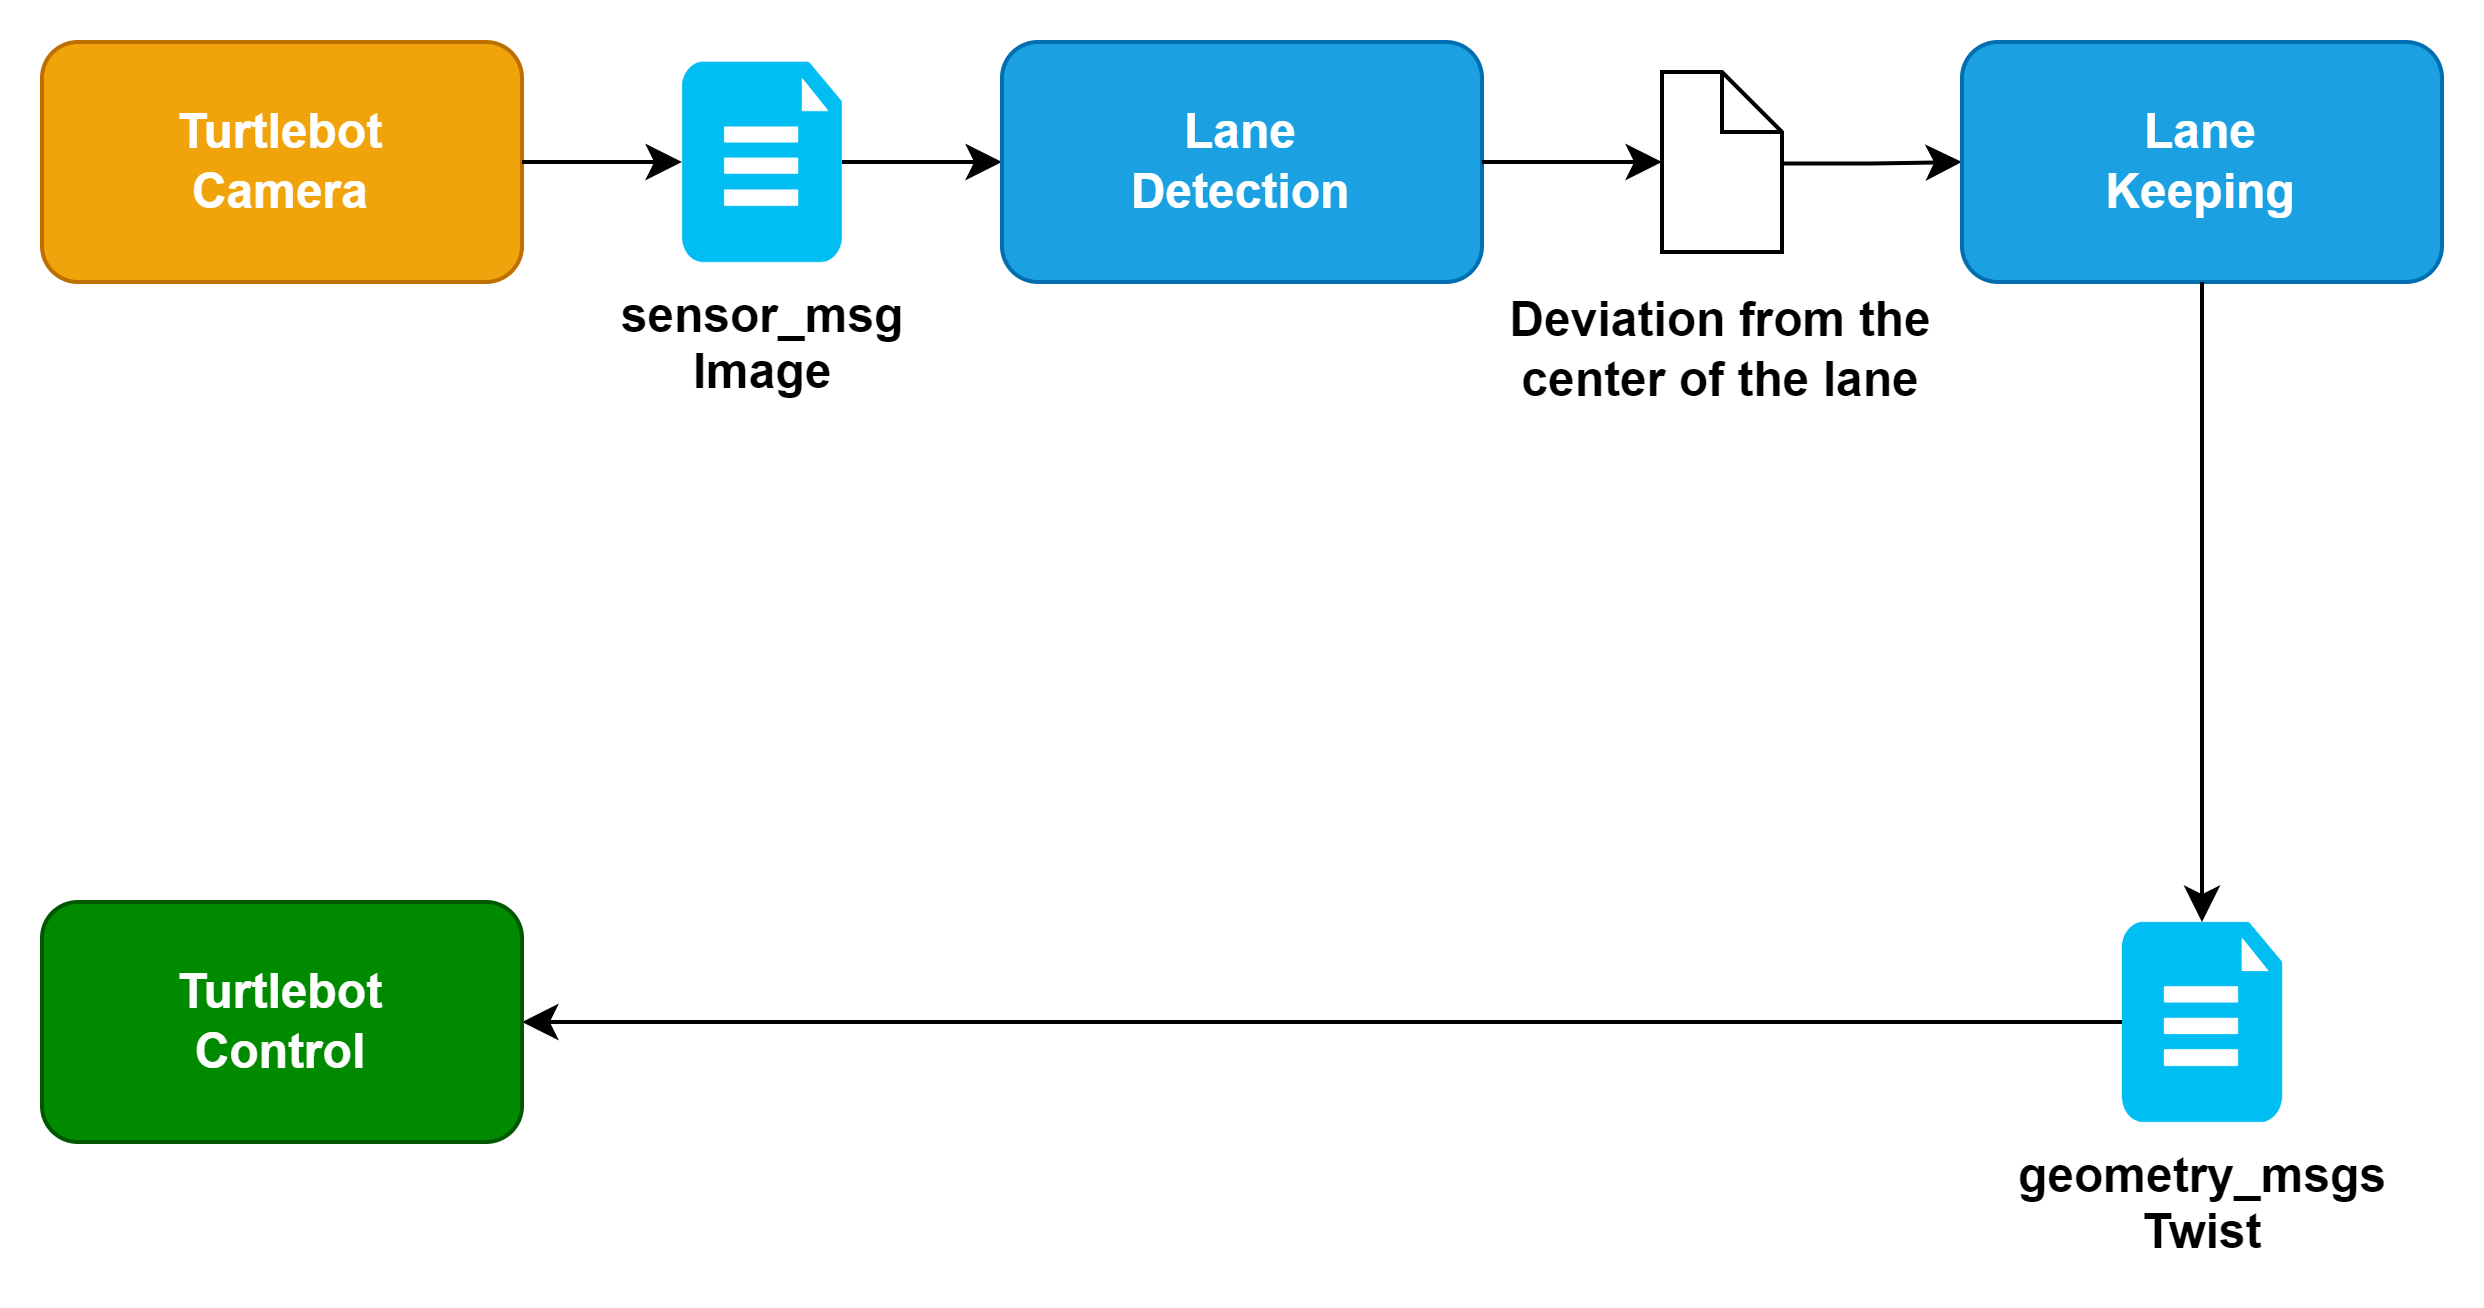
\includegraphics[width=\linewidth]{img/3_Architecture/general_arch.png}
    \captionof{figure}{Kiến trúc hệ thống}
\end{figure}

Trong đó các module hiện tại được hiện thực và có các chức năng sau:

\begin{itemize}
    \item \textbf{Module nhận diện làn đường:} Nhận đầu vào là ảnh trực tiếp từ camera, module sẽ xử lý và tìm hai phương trình làn đường \textbf{LL} (left\_lane), \textbf{RL}(right\_lane) đại diện cho hai làn đường và xác định độ lệch của robot so với tâm làn đường.
    \item \textbf{Module bám làn đường:} Đưa ra hành vi di chuyển của robot dựa vào kết quả thu thập được từ module phát hiện làn đường.
\end{itemize}

\section{Module nhận diện làn đường}

\subsection{Giới thiệu chức năng}

Module nhận diện làn đường là một trong những module nhận dữ liệu trực tiếp từ camera. Sau quá trình xử lý, module sẽ có được phương trình đường thẳng của hai làn đường được hai làn đường dự đoán và cung cấp thông tin cho hệ thống bám làn. Ngoài ra, Module nhận diện làn đường tương tác với Module bám làn đường để cung cấp thông tin vị trí của làn đường, ảnh hưởng đến quyết định lái xe.

\subsection{Mô tả chi tiết}
Module nhận diện làn đường như một hàm có tham số đầu vào và đầu ra như sau:
\begin{itemize}
    \item Input: Hình ảnh được trích xuất từ camera với kích cỡ 640 × 480 × 3
    \item Output: Độ lệch robot so với tâm làn đường.
\end{itemize}
Dữ liệu bên trong module sẽ đi qua các bước sau:
\newpage
\begin{figure}[!hbt]
    \centering
    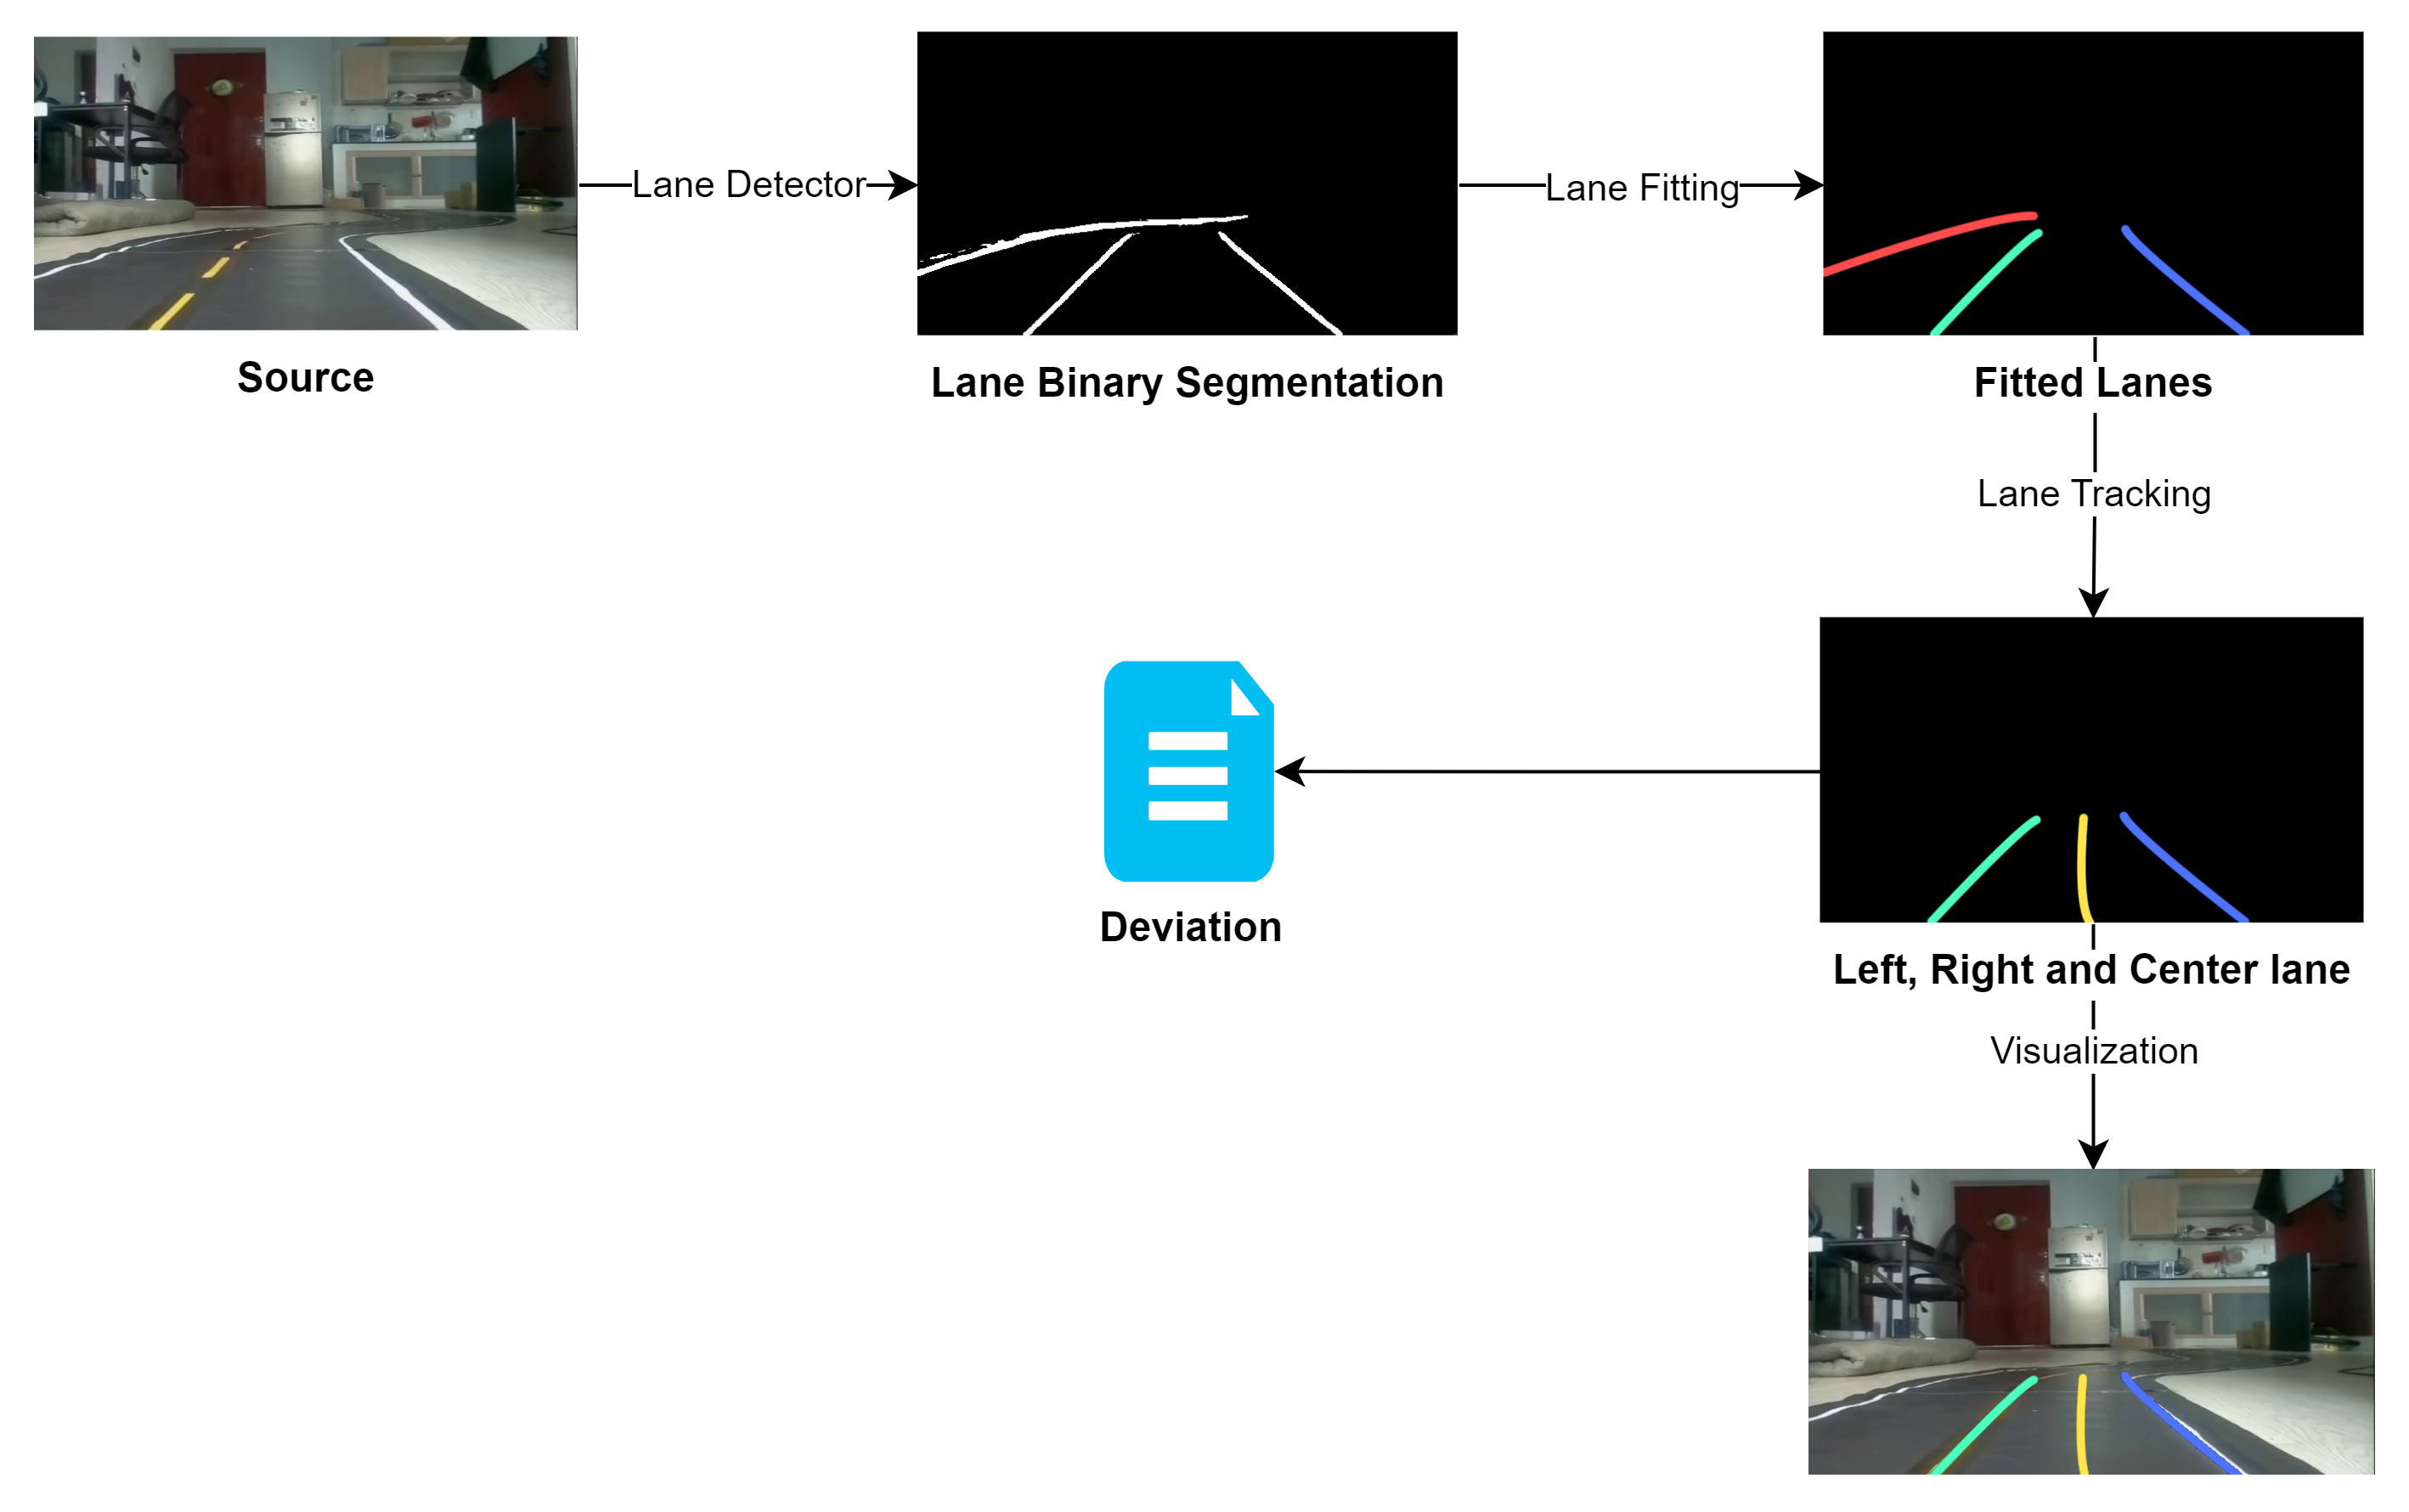
\includegraphics[width=15cm]{img/3_Architecture/lane_detector_arch.png}
    \captionof{figure}{Cấu trúc của module nhận diện làn đường}
\end{figure}

% TODO: Liệu có nên bỏ phần dưới đây

% \begin{itemize}
%     \item Model AI (khoảng 10ms với RTX4070 và CUDA 12.3): Segmentation những vùng có làn đường và trả về một bức ảnh dạng binary 640 x 360 x 1.
%     \item Backend: (khoảng 4ms): Sử dụng dữ liệu trả về bởi model, lọc những nhiễu và xử lý để cho ra phương trình đường thẳng hai làn đường và đưa ra thông tin độ lệch $d$ của robot so với tâm làn đường.
%     \item Hàm nhận diện làn đường trái phải có sử dụng thuật toán Hough Lines Transform\textsuperscript{\cite{houghtransform}} để phát hiện các đường thẳng và trả kết quả điểm đầu cuối. Sau đó, dựa vào điều kiện góc theta giữa các làn đường thẳng với trục hoành để phân loại chúng thành 01 làn đường trái và 01 làn đường phải (việc giải quyết bài toán này trong các trường hợp cụ thể sẽ được nêu rõ ở phần Backend chương 4). Khi xác định được 2 làn đường cụ thể, nhóm sẽ thu được kết quả tọa độ của 4 điểm TopLeft (TL), TopRight(TR), BottomLeft (BL), BottomRight(BR).

%     \item Hàm xác định độ lệch có chức năng tính toán độ lệch $d$ của robot so với tâm làn đường (với trường hợp cả làn trái và làn phải đều tồn tại) và trả về kết quả $d$ là thông tin vị trí robot cho module bám làn đường.
% \end{itemize}

\section{Module bám làn đường}

\subsection{Giới thiệu chức năng}

Mục tiêu chính của module này là điều khiển vận tốc và góc quay của robot sao cho nó giữ được vị trí trung tâm trên làn đường mong muốn.
\begin{enumerate}
    \item Ưu tiên việc chạy vào giữa mỗi làn để đảm bảo tối ưu được đường đi, và đúng luật giao thông
    \item Chạy được hết quãng đường và đạt đến đích trong một môi trường xác định, xử lý và đưa ra quyết định chỉ dựa vào các đầu vào sẵn có
    \item Trọng tâm của xe phải luôn được giữ bên trong làn đường.
\end{enumerate}
\subsection{Mô tả chi tiết}
\begin{figure}[htp]
    \centering
    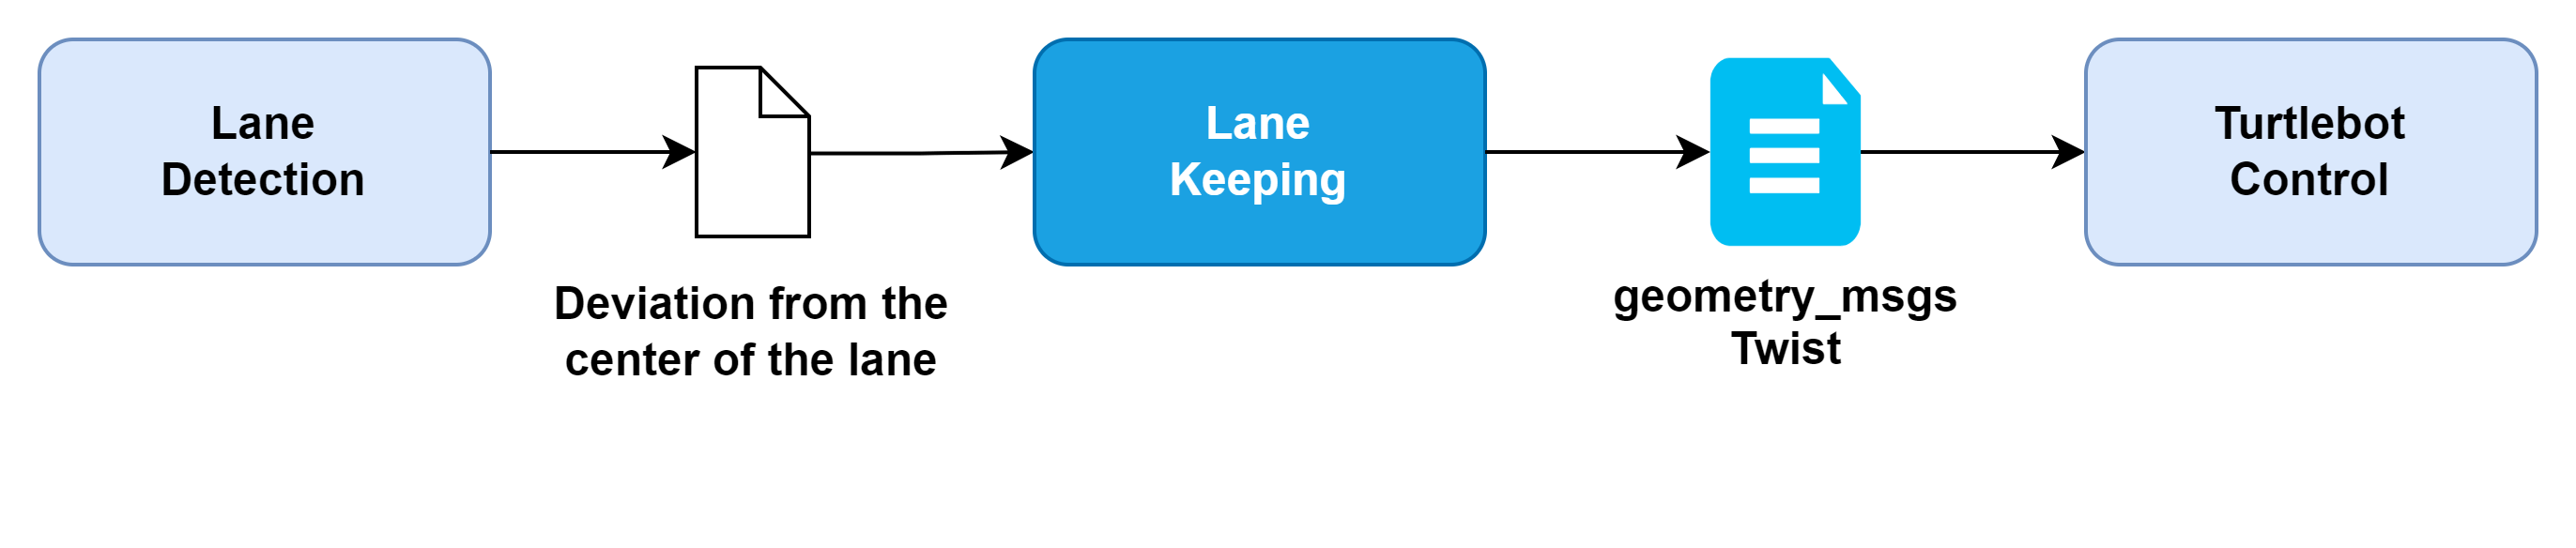
\includegraphics[width=\linewidth]{img/3_Architecture/lane_keeping_structure.png}
    \captionof{figure}{Cấu trúc của module bám làn đường}
\end{figure}

Module bám làn đường như một hàm có tham số đầu vào và đầu ra như sau:
\begin{itemize}
    \item \textbf{Input}:
    \begin{itemize}
        \item Độ lệch tâm làn đường: Tín hiệu này sẽ được gửi liên tục từ module phát hiện làn đường. Module này sẽ đảm bảo những tín hiệu gửi là đúng đắn, những tín hiệu lỗi sẽ được module nhận diện làn đường bỏ qua và gửi cảnh báo. Chính vì vậy, nếu không nhìn thấy làn đường trái hoặc phải, sẽ không trả về kết quả.
        \item Thông tin về độ lệch $d$ giữa tâm của robot so với tâm của làn đường 
    \end{itemize}
    \item \textbf{Output}: Output sẽ được gửi trực tiếp đến topic \textbf{cmd\_vel} nhằm điều khiển robot di chuyển:
    \begin{itemize}
        \item v\_linear: Vận tốc đi thẳng của robot (m/s)
        \item v\_angular: vận tốc xoay của robot (rad/s)
    \end{itemize}
\end{itemize}